\documentclass{beamer}
\usepackage{presentation}

\begin{document}

\frame{\titlepage}

\begin{frame}
  \frametitle{The prototype}

  \begin{columns}
    \column{0.5\textwidth}
    What worked
    \begin{itemize}
      \item SQLite3
      \item Persistence
      \item Web server
      \item Wi-Fi provisioning
    \end{itemize}

    \column{0.5\textwidth}
    What could be better
    \begin{itemize}
      \item MQTT
      \item LVGL: screen rendering
      \item SoC specs
      \item Device authentication
    \end{itemize}
  \end{columns}

  \note[item]{MQTT: persistent connection not possible --- mesage \textit{queue} not utilized}
  \note[item]{ESP32-C3: RISC-V SoCs do not support memory expansion}
  \note[item]{Disucss potential alternatives: Pi Zero 2W, ESP32-S3 }

\end{frame}

\begin{frame}
  \frametitle{Aesthetic rendering}

  \begin{center}
    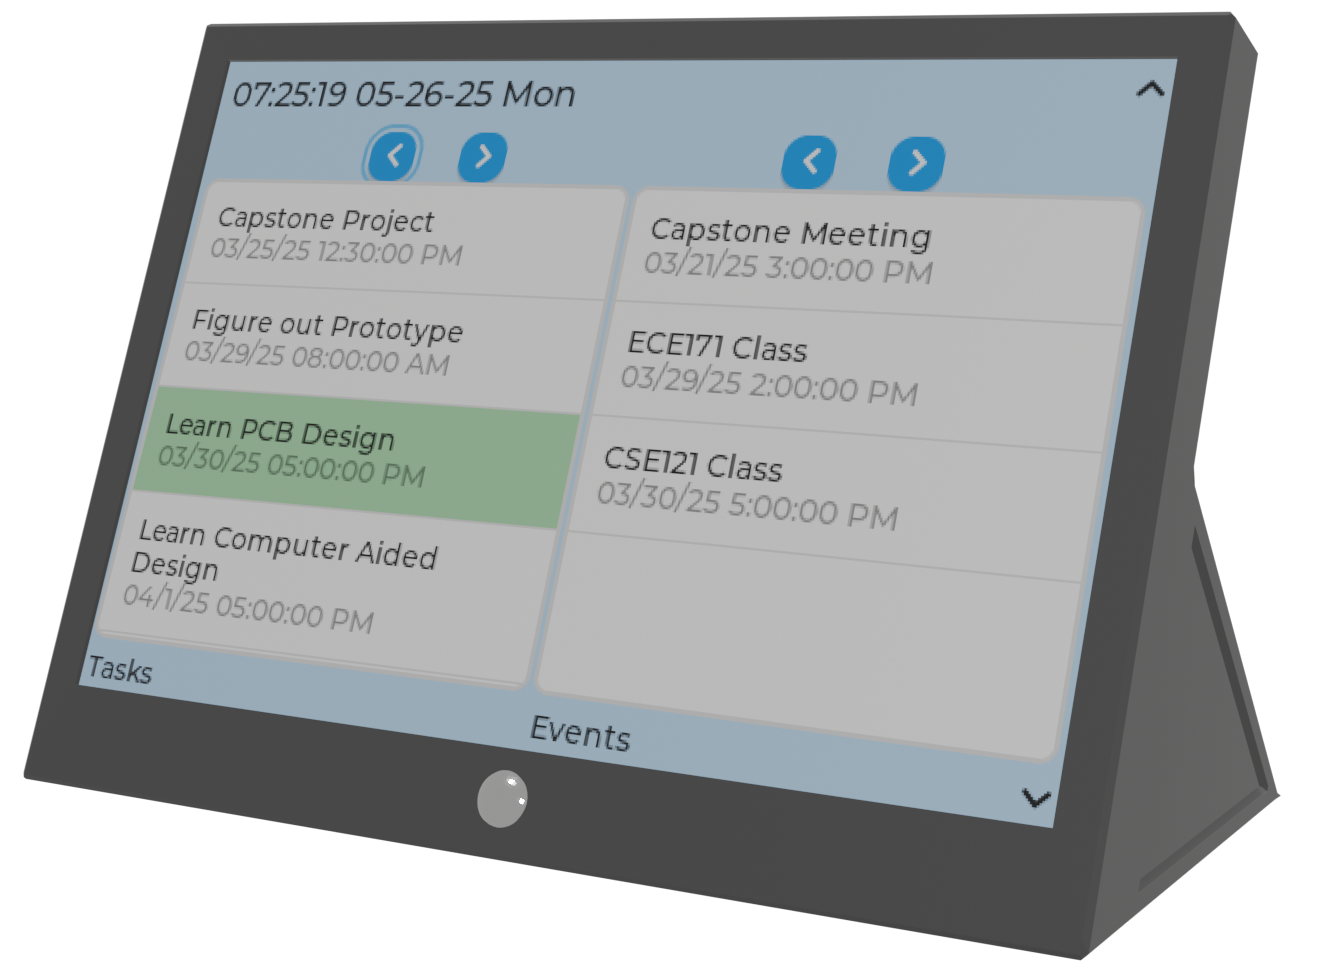
\includegraphics[width = 0.9 \textwidth]{schedule_companion_render.png}
  \end{center}

\end{frame}

\begin{frame}
  \frametitle{Server Architecture}

  \begin{center}
    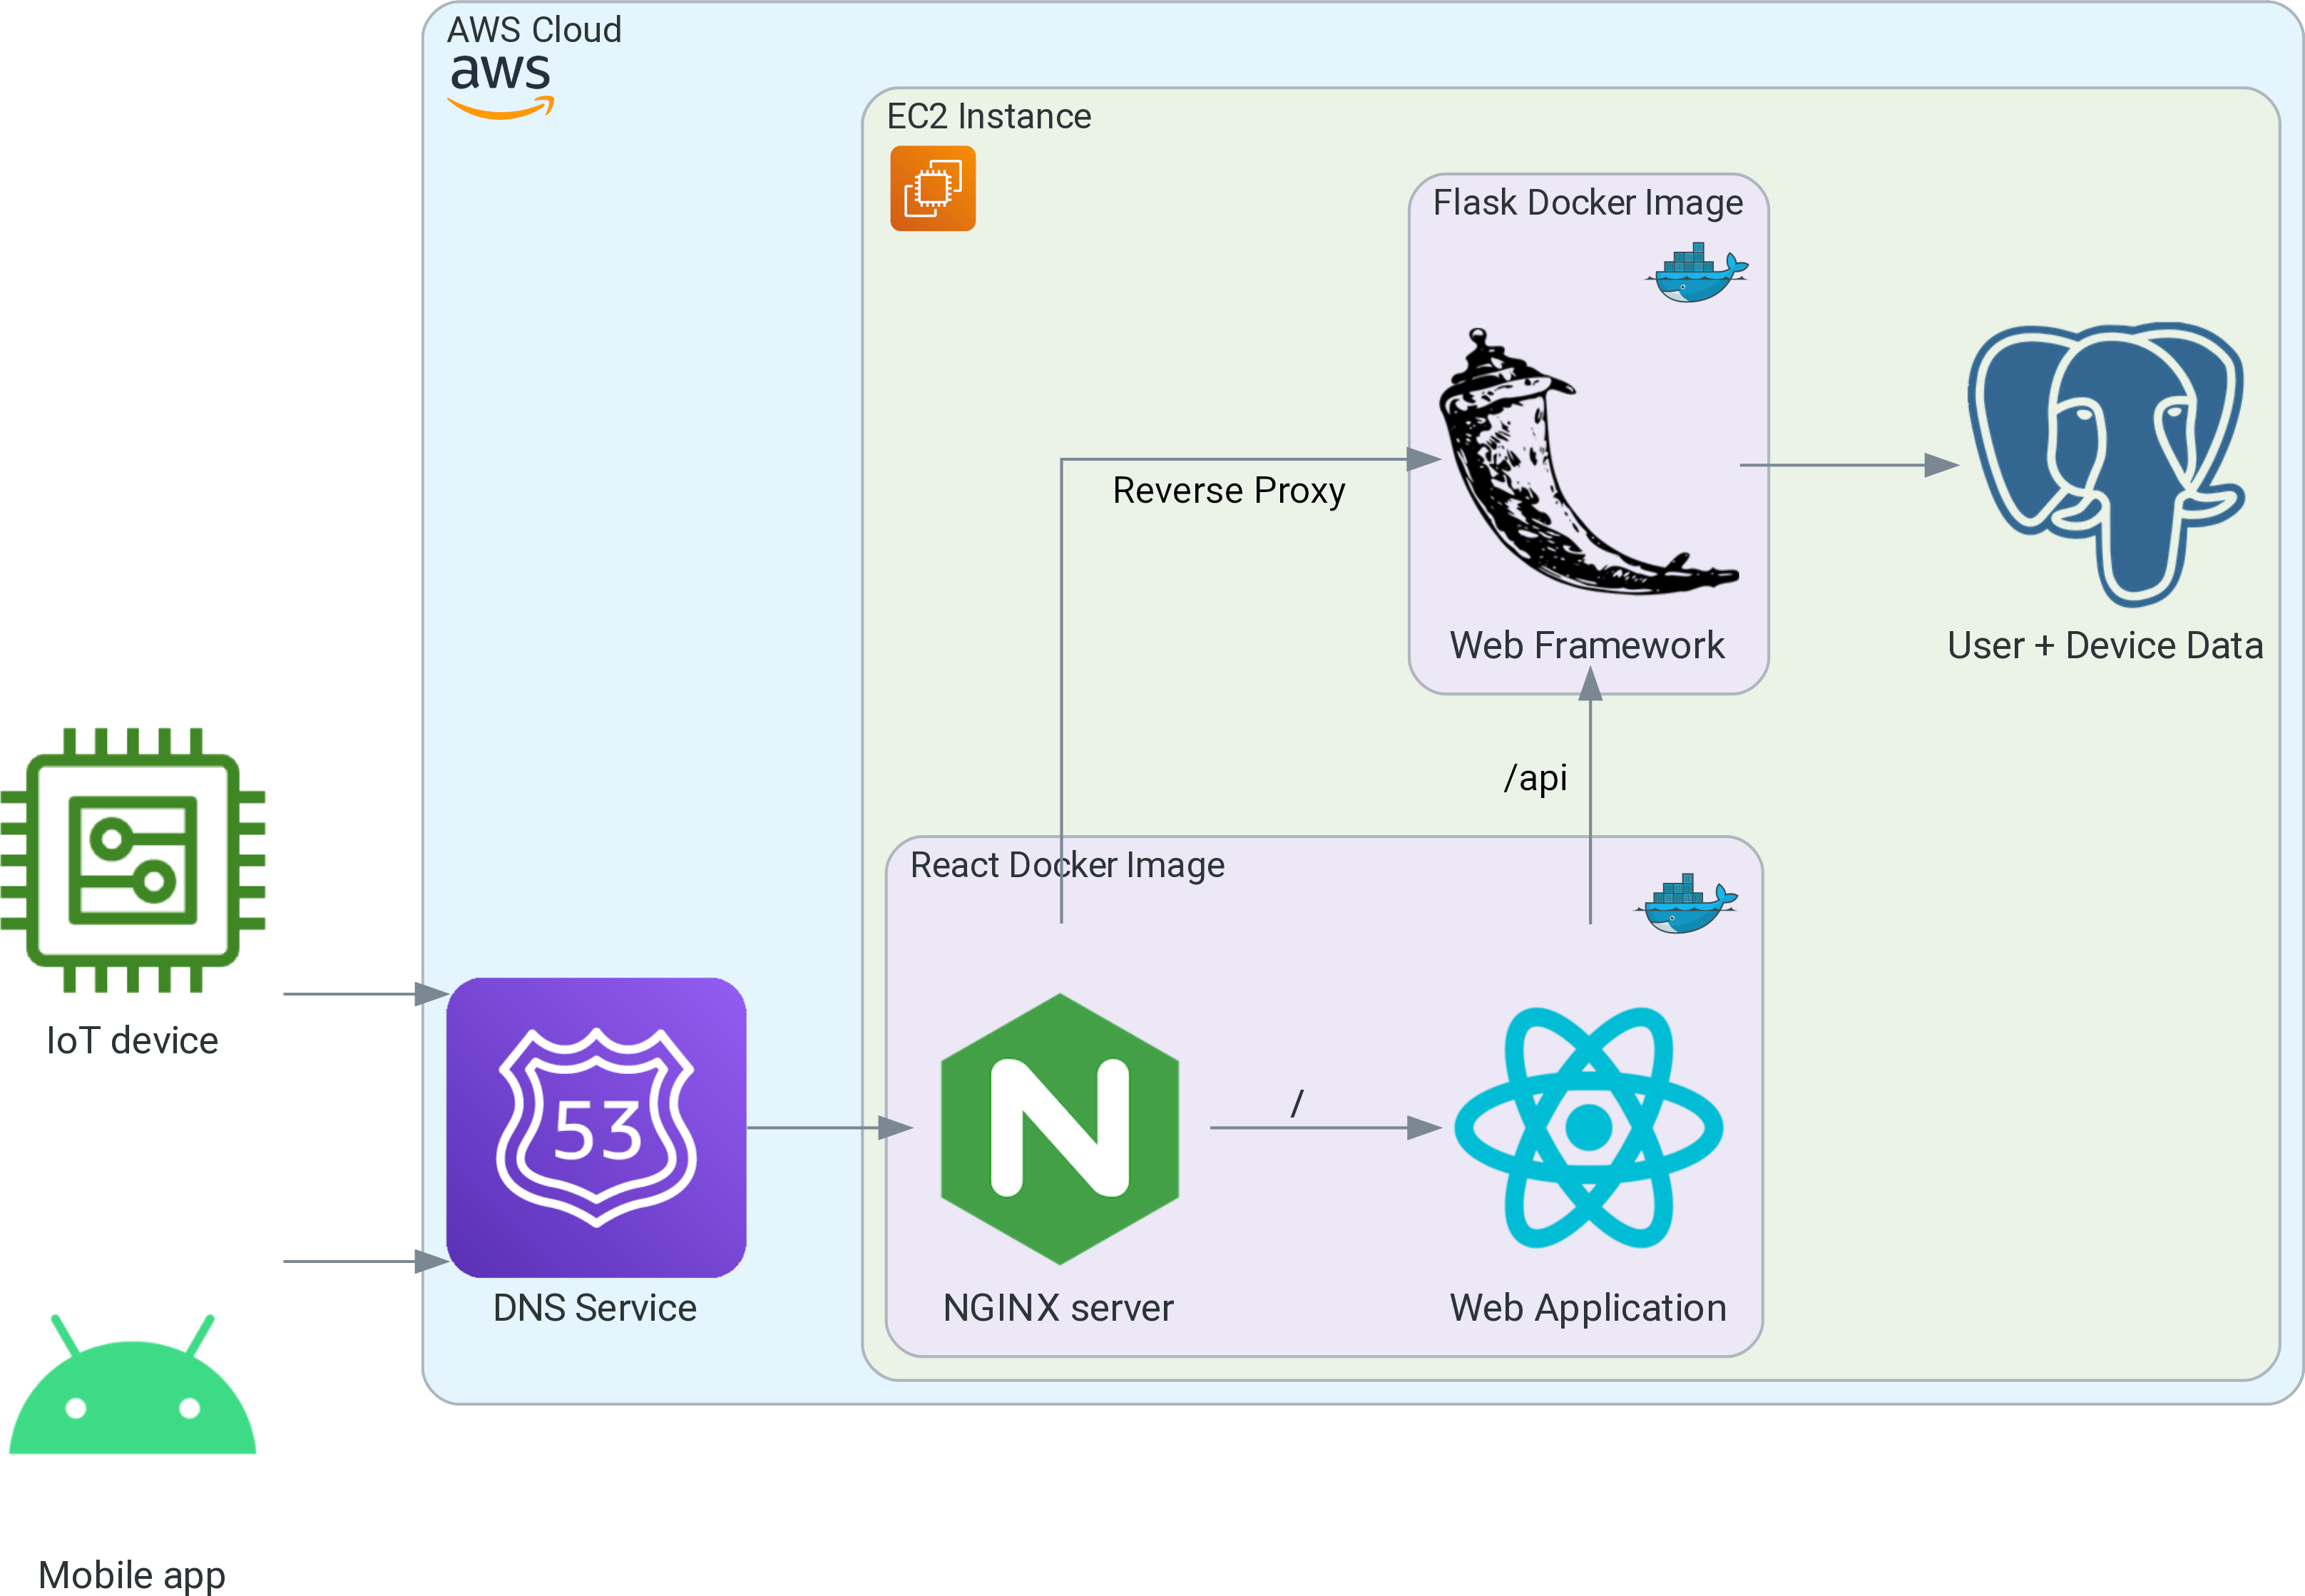
\includegraphics[width = 0.9 \textwidth]{data_flow.png}
  \end{center}

  \note[item]{React web app and the device will make requests to "/api" to interact with the server data}
  \note[item]{Both user and device will interact with the api after ensuring they have an un-expired jwt}
\end{frame}

\end{document}
